%% Преамбула TeX-файла

% 1. Стиль и язык
\documentclass{G7-32} % Стиль (по умолчанию размер шрифта 14pt)

% Остальные стандартные настройки убраны в preamble.inc.tex.
\sloppy

% Настройки стиля ГОСТ 7-32
% Для начала определяем, хотим мы или нет, чтобы рисунки и таблицы нумеровались в пределах раздела, или нам нужна сквозная нумерация.
\EqInChapter % формулы будут нумероваться в пределах раздела
\TableInChapter % таблицы будут нумероваться в пределах раздела
\PicInChapter % рисунки будут нумероваться в пределах раздела

% Добавляем гипертекстовое оглавление в PDF
\usepackage[
    bookmarks=true, colorlinks=true, unicode=true,
    allcolors=black,
]{hyperref}

\AfterHyperrefFix

\usepackage{microtype}% полезный пакет для микротипографии, увы под xelatex мало чего умеет, но под pdflatex хорошо улучшает читаемость

% Тире могут быть невидимы в Adobe Reader
\ifInvisibleDashes
    \MakeDashesBold
\fi

\usepackage{graphicx}

% Пакет Tikz
\usepackage{tikz}
\usetikzlibrary{arrows,positioning,shadows}

% Произвольная нумерация списков.
\usepackage{enumerate}

% ячейки в несколько строчек
\usepackage{multirow}

% itemize внутри tabular
\usepackage{paralist,array}

\setlength{\parskip}{0ex} % разрыв между абзацами

% Пакет для генерации случайного текста
\usepackage{blindtext}

% Центрирование подписей к плавающим окружениям
%\usepackage[justification=centering]{caption}

\usepackage{newfloat}
\DeclareFloatingEnvironment[
placement={!ht},
name=Equation
]{eqndescNoIndent}
\edef\fixEqndesc{\noexpand\setlength{\noexpand\parindent}{\the\parindent}\noexpand\setlength{\noexpand\parskip}{\the\parskip}}
\newenvironment{eqndesc}[1][!ht]{%
    \begin{eqndescNoIndent}[#1]%
\fixEqndesc%
}
{\end{eqndescNoIndent}}

% Подключаем пакет BibLaTeX для работы с библиографией
\usepackage[
parentracker=true,
style=gost-numeric,
bibstyle=gost-numeric,
language=auto,
autolang=other,
backend=biber,
sorting=none]{biblatex}
% Добавляем библиографию
\addbibresource{rpz.bib}
% Корректная обработка даты обращения в формате дд.мм.гг
\DeclareSourcemap{
    \maps{
        \map[overwrite]{
            \step[fieldsource=urldate,
            match=\regexp{([0-9]{2})\.([0-9]{2})\.([0-9]{4})},
            replace={$3-$2-$1},
            final]
        }
    }
}
% Убираем курсив из списка источников
\makeatletter
\renewrobustcmd*{\mkbibemph}{}
\protected\long\def\blx@imc@mkbibemph#1{#1}
\makeatother



% Настройки листингов.
\ifPDFTeX
    % 8 Листинги

\usepackage{listings}

% Значения по умолчанию
\lstset{
  basicstyle= \footnotesize,
  breakatwhitespace=true,% разрыв строк только на whitespacce
  breaklines=true,       % переносить длинные строки
% captionpos=b,          % подписи снизу -- вроде не надо
  inputencoding=utf8,
  numbers=left,          % нумерация слева
  numberstyle=\footnotesize,
  showspaces=false,      % показывать пробелы подчеркиваниями -- идиотизм 70-х годов
  showstringspaces=false,
  showtabs=false,        % и табы тоже
  stepnumber=1,
  tabsize=4,             % кому нужны табы по 8 символов?
  frame=single,
  extendedchars=\true,
  keepspaces=true
}

% Стиль для псевдокода: строчки обычно короткие, поэтому размер шрифта побольше
\lstdefinestyle{pseudocode}{
  basicstyle=\small,
  keywordstyle=\color{black}\bfseries\underbar,
  language=Pseudocode,
  numberstyle=\footnotesize,
  commentstyle=\footnotesize\it
}

% Стиль для обычного кода: маленький шрифт
\lstdefinestyle{realcode}{
  basicstyle=\scriptsize,
  numberstyle=\footnotesize
}

% Стиль для коротких кусков обычного кода: средний шрифт
\lstdefinestyle{simplecode}{
  basicstyle=\footnotesize,
  numberstyle=\footnotesize
}

% Стиль для BNF
\lstdefinestyle{grammar}{
  basicstyle=\footnotesize,
  numberstyle=\footnotesize,
  stringstyle=\bfseries\ttfamily,
  language=BNF
}

% Определим свой язык для написания псевдокодов на основе Python
\lstdefinelanguage[]{Pseudocode}[]{Python}{
  morekeywords={each,empty,wait,do},% ключевые слова добавлять сюда
  morecomment=[s]{\{}{\}},% комменты {а-ля Pascal} смотрятся нагляднее
  literate=% а сюда добавлять операторы, которые хотите отображать как мат. символы
    {->}{\ensuremath{$\rightarrow$}~}2%
    {<-}{\ensuremath{$\leftarrow$}~}2%
    {:=}{\ensuremath{$\leftarrow$}~}2%
    {<--}{\ensuremath{$\Longleftarrow$}~}2%
}[keywords,comments]

% Свой язык для задания грамматик в BNF
\lstdefinelanguage[]{BNF}[]{}{
  morekeywords={},
  morecomment=[s]{@}{@},
  morestring=[b]",%
  literate=%
    {->}{\ensuremath{$\rightarrow$}~}2%
    {*}{\ensuremath{$^*$}~}2%
    {+}{\ensuremath{$^+$}~}2%
    {|}{\ensuremath{$|$}~}2%
}[keywords,comments,strings]

% Подписи к листингам на русском языке.
\renewcommand\lstlistingname{Листинг}
\renewcommand\lstlistlistingname{Листинги}

\else
    \usepackage{local-minted}
\fi

% Стиль титульного листа и заголовки
\include{00-title}


\begin{document}

\frontmatter % выключает нумерацию ВСЕГО; здесь начинаются ненумерованные главы: реферат, введение, глоссарий, сокращения и прочее.

\maketitle %создает титульную страницу


\begin{executors}
\personalSignature{Первый исполнитель}{ФИО}

\personalSignature{Второй исполнитель}{ФИО}
\end{executors}


%\listoffigures                         % Список рисунков

%\listoftables                          % Список таблиц

%\NormRefs % Нормативные ссылки
% Команды \breakingbeforechapters и \nonbreakingbeforechapters
% управляют разрывом страницы перед главами.
% По-умолчанию страница разрывается.

% \nobreakingbeforechapters
% \breakingbeforechapters

\include{00-abstract}

\tableofcontents

\printnomenclature % Автоматический список сокращений

\include{12-intro}

\mainmatter % это включает нумерацию глав и секций в документе ниже

\chapter{Аналитический раздел}
\label{cha:analysis}
%
% % В начале раздела  можно напомнить его цель
%
В данном разделе анализируется и классифицируется существующая всячина и пути создания новой всячины. А вот отступ справа в 1 см. "--- это хоть и по ГОСТ, но ведь диагноз же...

\section{Анализ того и сего}

% Обратите внимание, что включается не ../dia/..., а inc/dia/...
% В Makefile есть соответствующее правило для inc/dia/*.pdf, которое
% берет исходные файлы из ../dia в этом случае.

\begin{figure}
  \centering
  
\includegraphics[width=\textwidth]{inc/dia/rpz-idef0}
  \caption{Рисунок}
  \label{fig:fig01}
\end{figure}

\begin{figure}
  \centering
  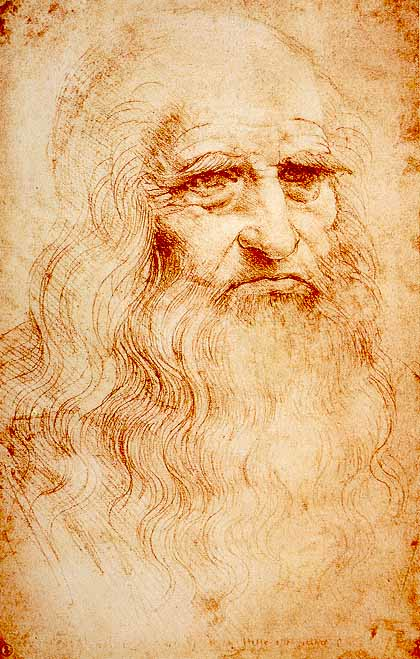
\includegraphics[height=0.85\textheight]{inc/img/leonardo}
  \caption{Предполагаемый автопортрет Леонардо да Винчи}
  \label{fig:leonardo}
\end{figure}

В \cite{Pup09} указано, что...

Кстати, про картинки. Во-первых, для фигур следует использовать \texttt{[ht]}. Если и после этого картинки вставляются <<не по ГОСТ>>, т.е. слишком далеко от места ссылки, "--- значит у вас в РПЗ \textbf{слишком мало текста}! Хотя и ужасный параметр \texttt{!ht} у окружения \texttt{figure} тоже никто не отменял, только при его использовании документ получается страшный, как в ворде, поэтому просьба так не делать по возможности.

\section{Существующие подходы к созданию всячины}

Известны следующие подходы...

\begin{enumerate}
\item Перечисление с номерами.
\item Номера первого уровня. Да, ГОСТ требует именно так "--- сначала буквы, на втором уровне "--- цифры.
Чуть ниже будет вариант <<нормальной>> нумерации и советы по её изменению.
Да, мне так нравится: на первом уровне выравнивание элементов как у обычных абзацев. Проверим теперь вложенные списки.
\begin{enumerate}
\item Номера второго уровня.
\item Номера второго уровня. Проверяем на длииииной-предлиииииииииинной строке, что получается.... Сойдёт.
\end{enumerate}
\item По мнению Лукьяненко, человеческий мозг старается подвести любую проблему к выбору
  из трех вариантов.
\item Четвёртый (и последний) элемент списка.
\end{enumerate}

Теперь мы покажем, как изменить нумерацию на «нормальную», если вам этого захочется. Пара команд в начале документа поможет нам.

\renewcommand{\labelenumi}{\arabic{enumi})}
\renewcommand{\labelenumii}{\asbuk{enumii})}

\begin{enumerate}
\item Изменим нумерацию на более привычную...
\item ... нарушим этим гост.
\begin{enumerate}
\item Но, пожалуй, так лучше.
\end{enumerate}
\end{enumerate}

В заключение покажем произвольные маркеры в списках. Для них нужен пакет \textbf{enumerate}.
\begin{enumerate}[1.]
\item Маркер с арабской цифрой и с точкой.
\item Маркер с арабской цифрой и с точкой.
\begin{enumerate}[I.]
\item Римская цифра с точкой.
\item Римская цифра с точкой.
\end{enumerate}
\end{enumerate}

В отчётах могут быть и таблицы "--- см. табл.~\ref{tab:tabular} и~\ref{tab:longtable}.
Небольшая таблица делается при помощи \textbf{tabular} внутри \textbf{table} (последний
полностью аналогичен \textbf{figure}, но добавляет другую подпись).

\begin{table}[ht]
  \caption{Пример короткой таблицы с коротким названием}
  \begin{tabular}{|r|c|c|c|l|}
  \hline
  Тело      & $F$ & $V$  & $E$ & $F+V-E-2$ \\
  \hline
  Тетраэдр  & 4   & 4    & 6   & 0         \\
  Куб       & 6   & 8    & 12  & 0         \\
  Октаэдр   & 8   & 6    & 12  & 0         \\
  Додекаэдр & 20  & 12   & 30  & 0         \\
  Икосаэдр  & 12  & 20   & 30  & 0         \\
  \hline
  Эйлер     & 666 & 9000 & 42  & $+\infty$ \\
  \hline
  \end{tabular}
  \label{tab:tabular}
\end{table}

Для больших таблиц следует использовать пакет \textbf{longtable}, позволяющий создавать
таблицы на несколько страниц по ГОСТ.

Для того, чтобы длинный текст разбивался на много строк в пределах одной ячейки, надо в
качестве ее формата задавать \texttt{p} и указывать явно ширину: в мм/дюймах
(\texttt{110mm}), относительно ширины страницы (\texttt{0.22\textbackslash textwidth})
и~т.п.

Можно также использовать уменьшенный шрифт "--- но, пожалуйста, тогда уж во \textbf{всей}
таблице сразу.

\begin{center}
  \begin{longtable}{|p{0.40\textwidth}|c|p{0.30\textwidth}|}
    \caption{Пример длинной таблицы с длинным названием на много длинных-длинных строк}
    \label{tab:longtable}
    \\ \hline
    Вид шума & Громкость, дБ & Комментарий \\
    \hline \endfirsthead
    \subcaption{Продолжение таблицы~\ref{tab:longtable}}
    \\ \hline \endhead
    \hline \subcaption{Продолжение на след. стр.}
    \endfoot
    \hline \endlastfoot
    Порог слышимости             & 0     &                                                \\
    \hline
    Шепот в тихой библиотеке     & 30    &                                                \\
    Обычный разговор             & 60-70 &                                                \\
    Звонок телефона              & 80    & \small{Конечно, это было до эпохи мобильников} \\
    Уличный шум                  & 85    & \small{(внутри машины)}                        \\
    Гудок поезда                 & 90    &                                                \\
    Шум электрички               & 95    &                                                \\
    \hline
    Порог здоровой нормы         & 90-95 & \small{Длительное пребывание на более
    громком шуме может привести к ухудшению слуха}                                        \\
    \hline
    Мотоцикл                     & 100   &                                                \\
    Power Mower                  & 107   & \small{(модель бензокосилки)}                  \\
    Бензопила                    & 110   & \small{(Doom в целом вреден для здоровья)}     \\
    Рок-концерт                  & 115   &                                                \\
    \hline
    Порог боли                   & 125   & \small{feel the pain}                          \\
    \hline
    Клепальный молоток           & 125   & \small{(автор сам не знает, что это)}          \\
    \hline
    Порог опасности              & 140   & \small{Даже кратковременное пребывание на
    шуме большего уровня может привести к необратимым последствиям}                       \\
    \hline
    Реактивный двигатель         & 140   &                                                \\
                                 & 180   & \small{Необратимое полное повреждение
                                 слуховых органов}                                        \\
    Самый громкий возможный звук & 194   & \small{Интересно, почему?..}                   \\
  \end{longtable}
\end{center}

%%% Local Variables:
%%% mode: latex
%%% TeX-master: "rpz"
%%% End:

\chapter{Конструкторский раздел}
\label{cha:design}

В данном разделе проектируется новая всячина.

\section{Архитектура всячины}

\subsection{Протестируем подпункт}
\subsubsection{А теперь подподпункт}


\paragraph{Проверка} параграфа. Вроде работает.
\paragraph{Вторая проверка} параграфа. Опять работает.

Вот.

\begin{itemize}
\item Это список с <<палочками>>.
\item Хотя он и по ГОСТ, но\dots
\end{itemize}

\begin{enumerate}
\item  Для списка, начинающегося с заглавной буквы, лучше список с цифрами.
\end{enumerate}

Формула \eqref{F:F1} совершено бессмысленна.

%Кстати, при каких-то условиях <<удавалось>> получить двойный скобки вокруг номеров формул. Вопрос исследуется.

\begin{equation}
a= cb
\label{F:F1}
\end{equation}

А формула~\eqref{eq:fourierrow} имеет некоторый смысл.
Кроме этого она пытается иллюстрировать применение окружения \textbf{eqndesc} которое размещает формулу совместно с её описанием.
Однако обратите внимание на нумерацию формул~\eqref{eq:fourierrow} и \eqref{F:F2}, попробуйте добавить \textbf{[H]} к такой формуле.

\begin{eqndesc}
    \begin{equation}\label{eq:fourierrow}
        f(x) = \frac{a_0}{2} + \sum\limits_{k=1}^{+\infty} A_k\cos\left(k\frac{2\pi}{\tau}x+\theta_k\right)
    \end{equation}

    где $A_k$ "--- амплитуда  k-го гармонического колебания,\\
    $A_k$ "--- амплитуда $k$-го гармонического колебания,\\
    $ k\frac{2\pi}{\tau} = k\omega$ "--- круговая частота гармонического колебания,\\
    $\theta_k$ "--- начальная фаза $k$-го колебания.
\end{eqndesc}


Окружение \texttt{cases} опять работает (см. \eqref{F:F2}), спасибо И. Короткову за исправления..


\begin{equation}
a= \begin{cases}
 3x + 5y + z, \mbox{если хорошо} \\
 7x - 2y + 4z, \mbox{если плохо}\\
 -6x + 3y + 2z, \mbox{если совсем плохо}
\end{cases}
\label{F:F2}
\end{equation}

\section{Подсистема всякой ерунды}

Культурная вставка dot-файлов через утилиту dot2tex (рис.~\ref{fig:fig02}).

\begin{figure}
  \centering
% [width=0.5\textwidth] --- регулировка ширины картинки
  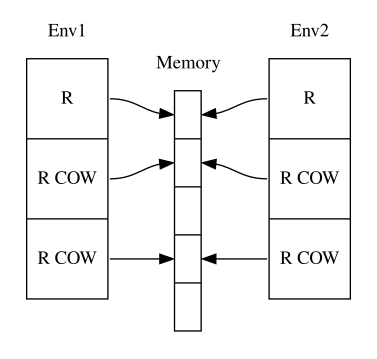
\includegraphics[width=.5\textwidth]{inc/dot/cow2}
  \caption{Рисунок}
  \label{fig:fig02}
\end{figure}


\subsection{Блок-схема всякой ерунды}

\subsubsection*{Кстати о заголовках}

У нас есть и \textbf{subsubsection}. Только лучше её не нумеровать.

%%% Local Variables:
%%% mode: latex
%%% TeX-master: "rpz"
%%% End:

\chapter{Технологический раздел}
\label{cha:impl}

В данном разделе описано изготовление и требование всячины. Кстати,
в Latex нужно эскейпить подчёркивание (писать <<\verb|some\_function|>> для \textbf{some\_function}).

\ifPDFTeX
    Для вставки кода есть пакет \textbf{listings}. К сожалению, пакет \textbf{listings} всё ещё
    работает криво при появлении в листинге русских букв и кодировке исходников utf-8.
    В данном примере он (увы) на лету конвертируется в koi-8 в ходе сборки pdf.

    Есть альтернатива \textbf{listingsutf8}, однако она работает лишь с
    \textbf{\textbackslash{}lstinputlisting}, но не с окружением \textbf{\textbackslash{}lstlisting}

    Вот так можно вставлять псевдокод (питоноподобный язык определен в \textbf{listings.inc.tex}):

    \begin{lstlisting}[style=pseudocode,caption={Алгоритм оценки дипломных работ}]
def EvaluateDiplomas():
    for each student in Masters:
        student.Mark := 5
    for each student in Engineers:
        if Good(student):
            student.Mark := 5
        else:
            student.Mark := 4
    \end{lstlisting}

    Еще в шаблоне определен псевдоязык для BNF:

    \begin{lstlisting}[style=grammar,basicstyle=\small,caption={Грамматика}]
ifstmt -> "if" "(" expression ")" stmt |
        "if" "(" expression ")" stmt1 "else" stmt2
number -> digit digit*
    \end{lstlisting}

    В листинге~\ref{lst:sample01} работают русские буквы. Сильная магия. Однако, работает
    только во включаемых файлах, прямо в \TeX{} нельзя.

    \lstinputlisting[language=C,caption=Пример (\textbf{test.c}),label=lst:sample01]{inc/src/test.c}

    \lstinputlisting[language=Python]{inc/src/get_presentation.py}

\else

    Для вставки кода есть пакет \texttt{minted}. Он хорош всем кроме: необходимости
    Python (есть во всех нормальных (нет, Windows, я не про тебя) ОС) и Pygments и
    того, что нормально работает лишь в \XeLaTeX.

    \ifdefined\NoMinted
        Но к сожалению, у вас, по-видимому, не установлен Python или pygmentize.
    \else
        Можно пользоваться расширенным BFN:

        \begin{listing}[H]
            \begin{ebnfcode}
letter = "A" | "B" | "C" | "D" | "E" | "F" | "G"
       | "H" | "I" | "J" | "K" | "L" | "M" | "N"
       | "O" | "P" | "Q" | "R" | "S" | "T" | "U"
       | "V" | "W" | "X" | "Y" | "Z" ;
digit = "0" | "1" | "2" | "3" | "4" | "5" | "6" | "7" | "8" | "9" ;
symbol = "[" | "]" | "{" | "}" | "(" | ")" | "<" | ">"
       | "'" | '"' | "=" | "|" | "." | "," | ";" ;
character = letter | digit | symbol | "_" ;

identifier = letter , { letter | digit | "_" } ;
terminal = "'" , character , { character } , "'"
         | '"' , character , { character } , '"' ;

lhs = identifier ;
rhs = identifier
     | terminal
     | "[" , rhs , "]"
     | "{" , rhs , "}"
     | "(" , rhs , ")"
     | rhs , "|" , rhs
     | rhs , "," , rhs ;

rule = lhs , "=" , rhs , ";" ;
grammar = { rule } ;
            \end{ebnfcode}
            \caption{EBNF определённый через EBNF}
            \label{lst:ebnf}
        \end{listing}

        А вот в листинге \ref{lst:c} на языке C работают русские комменты. Спасибо
        Pygments и Minted за это.

        \begin{listing}[H]
            \cfile{inc/src/test.c}
            \caption{Пример — test.c}
        \end{listing}
        \label{lst:c}

        \begin{listing}[H]
            \pythonfile{inc/src/get_presentation.py}
            \caption{Пример Python кода}\label{lst:py}
        \end{listing}

    \fi
\fi
% Для вставки реального кода лучше использовать \texttt{\textbackslash lstinputlisting} (который понимает
% UTF8) и стили \textbf{realcode} либо \textbf{simplecode} (в зависимости от размера куска).

Можно также использовать окружение \textbf{verbatim}, если \textbf{listings} чем-то не
устраивает. Только следует помнить, что табы в нём <<съедаются>>. Существует так же команда \textbf{\textbackslash{}verbatiminput} для вставки файла.

\begin{verbatim}
a_b = a + b; // русский комментарий
if (a_b > 0)
    a_b = 0;
\end{verbatim}

%%% Local Variables:
%%% mode: latex
%%% TeX-master: "rpz"
%%% End:

\include{50-research}
\include{60-economics}
\include{70-bzd}

\backmatter %% Здесь заканчивается нумерованная часть документа и начинаются ссылки и

\include{80-conclusion}%% заключение


% % Список литературы при помощи BibTeX
% Юзать так:
%
% pdflatex rpz
% bibtex rpz
% pdflatex rpz

%\bibliographystyle{ugost2008}
%\bibliography{rpz}
\printbibliography[title=Список использованных источников]
%%% Local Variables: 
%%% mode: latex
%%% TeX-master: "rpz"
%%% End: 



\appendix   % Тут идут приложения

\include{90-appendix1}

\include{91-appendix2}

\end{document}

%%% Local Variables:
%%% mode: latex
%%% TeX-master: t
%%% End:
